This chapter will include the discussion of the key areas of this thesis. This includes...

\section{Choice of Ensemble Factors}
The choice of object size and image quality as the deciding factors on how to create different ensemble members were made to address both challenges in object detection within object and image variations. The decision to use object size was clear as detectors results on benchmarks such as \gls{mscoco} showed that smaller objects are more difficult to detect. However, limited work has been done on image quality factors and object detection. Therefore, this was a more experimental part of the ensemble design. In regards to object size, the use of a trained \gls{rpn} is a strong and easy approach to use. However, the \gls{rpn} was trained to detect objects of all sizes. Rather it could have been possible to train an \gls{rpn} towards object sizes using the ground truth annotations such that each of the network ensemble were fed with region proposals from a better starting point. This could of course lead to issues in the ensemble as it would put a challenge on ensuring the ensemble members are combining results on the same object at test time. The choice of \gls{iqa} for the measurement of image quality may have a number of drawbacks. Firstly methods within \gls{iqa} attempt to estimate the subjective quality rather than objective. If image quality is a factor in object detection it would be due to the objective distortions present in an image, not that subjective evaluation of a person. Therefore, a method an objective method for measuring distortions in an image may be more appropriate. However, as the goal is ensemble methods is to reduce the variance in training the use of \gls{iqa} methods can still be suitable. Especially, if used in a systematic method as in this work.


\section{Choice of Object Detector}
The requirements set out in this work for the choice of the object detector was that it should be state-of-the-art \gls{cnn}-based. Three options were found, namely, Faster R-CNN, \gls{rfcn} and YOLOv2. Through both an analysis of the technical aspects and results of the three it was determined that a detector with ResNets as the backbone model should be used. Due to GPU limitations, the decision was made to use the \gls{rfcn}, however, any of the three could have been used. The overall goal of the thesis was to see if a \gls{cnn}-based object detector could be aided by ensemble methods chosen by robust-related challenges. Therefore, any of the detectors could have been used, as an assumption can be made that the benefits or limitations of the ensemble is equally applicable regardless of the choice.

\section{Training the Ensemble}
This section will discuss the process of training the ensemble members. This includes creating the data subsets for each member, the training of the \glspl{cnn} and.... \add[inline]{what is discussed}

\subsection{Creating the Data Subsets}
As mentioned, the aim of training multiple \glspl{rfcn} on different subsets of data was to decrease the overall variance in comparison to a model trained on all of the training data. Therefore, by measuring both object size and image quality factors on the 07++12 datasets the distributions of the data was the leading reason for how the subsets would be created. In all cases, apart from JPEG and JP2K compression, the distribution was heavily skewed towards lower numbers. As the requirement in the splitting of data was the subsets should have even number of ground truth examples this creating uneven datasets in regards to their variance. This choice leads to models within an ensemble factor which could vary greatly in terms of variance. There are potential positives and negatives to this. Firstly, by training two models the variance is already decreased as each model covers their own subset. However, one of these models has minimal variance and has to potential to be a powerful expert member. Issues with this are that the models are not trained under the same conditions which could lead to problems in the ensemble process. Which was attempted to be addressed by the weighted averaging combination process.
\\\\
Another issue when creating the datasets is ground truth examples for a given class may be skewed towards one of the two models. This can be seen in the examples of object size for the classes car (class 7) and cat (class 8) in \figref{classskew}. The distribution of ground truth object sizes is very different between the two classes. Cars in 07++12 tend to be of much smaller object size and is similar to the size distribution for all objects. Whereas, the cat class sizes are much more evenly distributed  However, the threshold for determining the split in data of 19,205.5 was found using the median size across all object sizes. Therefore, the number of cat training examples is much larger in this subset of larger ground truth examples. This could lead to the smaller resolution model not being able to generalise well towards images of this class.


\begin{figure}[H]
    \centering
    \begin{subfigure}[b]{0.45\textwidth}
        \center
        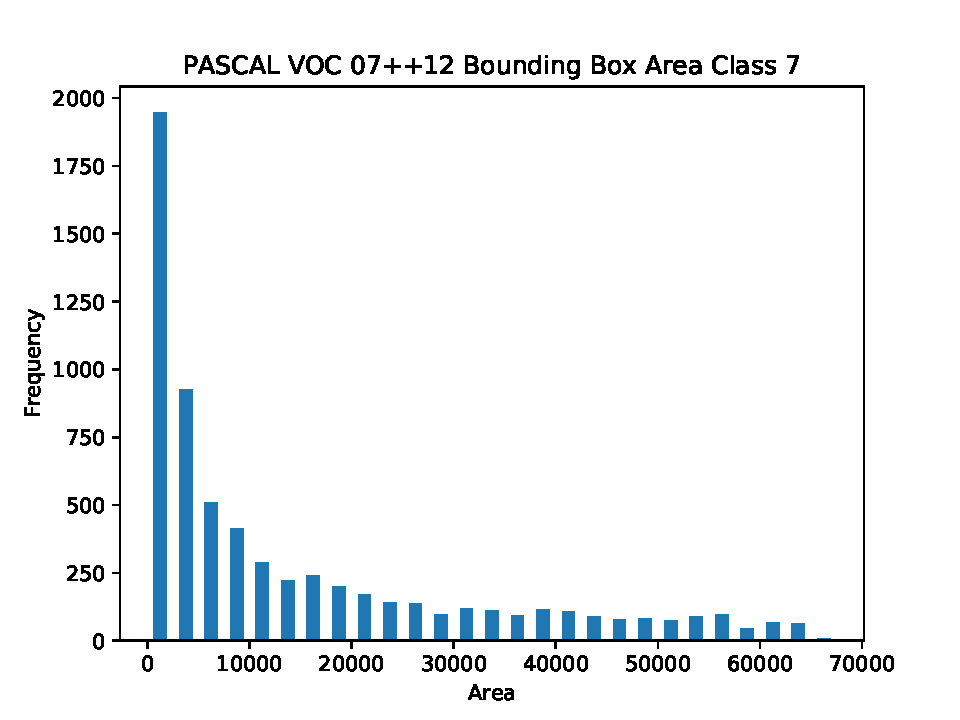
\includegraphics[width=\textwidth]{Figs/Conclusion/trainvalhist_class7.pdf}
        \caption{}\label{fig:}
    \end{subfigure}
    \begin{subfigure}[b]{0.45\textwidth}
        \center
        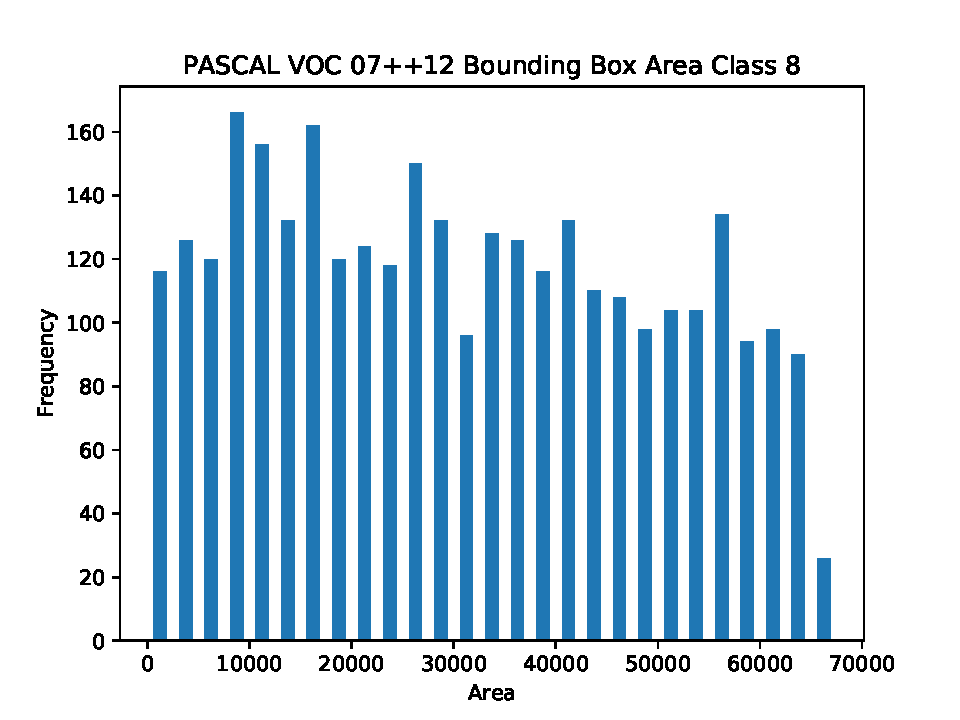
\includegraphics[width=\textwidth]{Figs/Conclusion/trainvalhist_class8.pdf}
        \caption{}\label{fig:}
    \end{subfigure}
    \caption{Differences in distribution of ground truth object sizes for the classes car (a) and cat (b) in 07++12.}
    \label{fig:classskew}
\end{figure} 

A potential solution to both issues in the creation of the data subsets is to use augmented data. The use of such data is a common strategy in training \glspl{cnn}, with horizontal flipping of ground truths being used in this project. Data could however be augmented towards evening the differences in distributions in both cases. For example, by interpolating smaller ground truth objects to larger resolutions. However, an issue with this example is that interpolation methods can produce additional distortions in the form of artefacts if images are scaled to a large degree.

\subsection{Training \gls{rfcn} Members}
The training of the individual \gls{rfcn} ensemble members was kept constant such that the effect of different data sampling and selection could be evaluated. However, as seen in other works \gls{cnn}-based object detectors can be trained with different architectural considerations and after combined in an ensemble \cite{deepres}. Therefore, another option could have been to vary the \glspl{rfcn} such as with different filter sizes, loss functions or depth of the networks. These networks could then be tested on a validation set to find complementary networks for an ensemble.

\section{Ensemble Combination}